\documentclass[journal, a4paper]{IEEEtran}
\usepackage{cite}
\usepackage{amsmath,amssymb,amsfonts}
\usepackage{graphicx}
\usepackage{textcomp}
\usepackage{xcolor}
\usepackage{float}

\begin{document}

\title{Explaining the Black Box: A Study on the Application of Explainable Artificial Intelligence (XAI) Techniques to Machine Learning Models}
\author{
    \large
    \IEEEauthorblockN{Magdalena~Pakuła\IEEEauthorrefmark{1}}
    and
    \IEEEauthorblockN{Jakub~Pawlak\IEEEauthorrefmark{2}}\\[1ex]
    \normalsize
    \IEEEauthorblockA{
        WFTIMS, Politechnika Łódzka\\
        Email: \IEEEauthorrefmark{1}254220@edu.p.lodz.pl, \IEEEauthorrefmark{2}254222@edu.p.lodz.pl
    }
}


\maketitle

\begin{abstract}
    The increasing reliance on artificial neural networks in various applications has raised concerns about their \textit{black box} nature, making it challenging to understand the decision-making processes behind their predictions.
    This report addresses this challenge by exploring the application of so-called Explainable Artificial Intelligence (XAI) techniques to machine learning models.
    Specifically, we employ local explanation approaches, including attributions and counterfactual examples, using the Captum library in the PyTorch such as LIME, saliency maps or integrated gradients techniques.
    Our study aims to shed light on the previously trained models, providing a deeper understanding of how they make predictions and present those findings in this report
\end{abstract}

\section{Introduction}\label{sec:introduction}

\IEEEPARstart{A}{rtificial} neural networks (ANNs) have revolutionized various industries and applications, from healthcare to finance, by enabling accurate predictions and decision-making.
However, the increasing reliance on these models has also raised concerns about their \textit{black box} nature, making it challenging to understand the decision-making processes behind their predictions.
This opacity can lead to a lack of trust in the models, as well as difficulties in identifying biases and errors.
To address this challenge, Explainable Artificial Intelligence (XAI) techniques have emerged as a crucial step towards building more transparent and accountable machine learning models.
By applying XAI methods, we can gain insights into the internal workings of complex models, providing a deeper understanding of how they make predictions and enabling more informed decision-making.
This project aims to explore the application of XAI techniques to machine learning models, specifically focusing on local explanation approaches such as attributions and counterfactual examples.
By shedding light on the previously trained models, we aim to provide a better understanding of how they make predictions and contribute to the development of more transparent and trustworthy AI systems.

\section{Related Work}\label{sec:related-work}
During this study, we explored various methods used to enhance the interpretability and transparency of ANNs through XAI techniques.
The first paper in this domain we examined was~\cite{ribeiro2016should} by Ribeiro et al.
This paper was the first to publicly introduce the Local Interpretable Model-Agnostic Explanations (LIME) framework, which generates local, interpretable explanations for the predictions of any machine learning model.
The key idea behind LIME is to approximate the original complex model with an interpretable model that is locally faithful to the prediction of interest.
This paper was an important step in the development of XAI techniques, as it demonstrated the feasibility and utility of interpretable explanations.
Since then, the field of XAI has continued to evolve, with many other techniques (e.g. SHAP, TCAV, GradCAM) being proposed to enhance the transparency and interpretability of AI systems.
However, LIME provides local explanations that are specific to individual predictions and while useful, these local explanations may not offer a comprehensive understanding of the model's overall behavior~\cite{NIPS2017_8a20a862}.

Different approach for understanding model predictions are saliency maps thoroughly explained by Simonyan et al.~\cite{Simonyan14a}.
This paper presents the method, which computes the gradient of the score of the predicted class with respect to the input image.
The gradient essentially measures how small changes in each pixel value of the image will affect the output score.
The absolute values of these gradients are taken to represent the importance of each pixel and pixels with larger gradient magnitudes are considered more important for the classification decision.
Therefore, saliency maps effectively highlight discriminative image regions and objects, which are easily interpretable by a human eye.
Such examples are shown and prove the usefulness of this method.

To have a broader view and better understanding using another method we reviewed another influential paper by Sundararajan et al.~\cite{ribeiro2016should}, which provided an alternative surrogate-based methods like LIME or sometimes misleading saliency maps~\cite{adebayo2018sanity}.
The authors introduce and demonstrate the usefulness of Integrated Gradients through various case studies, including image classification.
They show that this method can provide meaningful and intuitive explanations of the model's predictions, which can be valuable for tasks like feature importance analysis.
Additionally, the authors compare Integrated Gradients method to other gradient-based attribution methods, such as Saliency Maps and Deconvolution, and highlight the advantages of it in terms of satisfying desirable properties for explanations.

Furthermore, counterfactuals are an essential aspect of XAI, as they provide a way to evaluate the robustness of a model's predictions by considering what would have happened if certain conditions had been different~\cite{adebayo2018sanity}.
This is particularly important in high-stakes applications, such as healthcare or finance, where the consequences of incorrect predictions can be severe.
For example, Adebayo et al.~\cite{adebayo2018sanity} evaluated the reliability of saliency maps on the MNIST and CIFAR-10 image classification datasets by applying counterfactual perturbations like rotation and occlusion to the input images.
They found that many popular saliency map methods failed to provide faithful explanations, underscoring the importance of using counterfactuals to assess the robustness of model predictions.

Those papers provide a solid ground for experimenting on different models with different methods in order to fully understand models predictions.
\section{Methods}\label{sec:methodology}

This experiment will be conducted on various types of data and ANN models for testing the versatility of different XAI methods.
Models used in this experiment are:
\begin{itemize}
    \item Three MLP models for classifying iris flowers, distinguishing wines and diagnosing breast cancer
    \item Three MLP models for classifying handwritten numbers from the MNIST dataset
    \item CNN model for the MNIST dataset
    \item CNN model for distinguishing objects in images from the CIFAR10 dataset
\end{itemize}

After thoroughly reviewing research paper, we decided to firstly understand what was important in making a decision for a specific input by finding attributions and counterfacts using the following methods:

\begin{itemize}
    \item \textbf{LIME:}
    is a model-agnostic technique that explains the predictions of any classifier by learning an interpretable model locally around the prediction.
    It approximates the decision boundary around a given input \( \mathbf{x} \) using a linear regression model:
    \[
    f(\mathbf{x}') = \boldsymbol{\theta} \cdot \mathbf{x}' + b
    \]
    where \( \boldsymbol{\theta} \) are the coefficients of the linear model and \( b \) is the bias term.
    By analyzing \( \boldsymbol{\theta} \), LIME identifies the important features that influenced the prediction \( f(\mathbf{x}') \).

    \item \textbf{Saliency Maps:}
    highlight input features that are most influential for a model's prediction.
    They are computed by taking the absolute gradients of the output \( f(\mathbf{x}) \) with respect to the input \( \mathbf{x} \):
    \[
    S(\mathbf{x}) = \left|\frac{\partial f(\mathbf{x})}{\partial \mathbf{x}}\right|
    \]
    These maps provide insights into how sensitive the model's output is to changes in each input feature \( \mathbf{x}_i \).

    \item \textbf{Integrated Gradients:}
    attribute an output prediction to input features by integrating the gradients of the output \( f(\mathbf{x}) \) with respect to the input \( \mathbf{x} \) along a linear path from a baseline input \( \mathbf{x}' \) to the actual input \( \mathbf{x} \):
    \[
    \phi_i(\mathbf{x}) = (x_i - x'_i) \cdot \int_{\alpha=0}^{1} \frac{\partial f(\mathbf{x}' + \alpha (\mathbf{x} - \mathbf{x}'))}{\partial \mathbf{x}_i} \, d\alpha
    \]
    This method provides a comprehensive attribution of the model's prediction to each feature \( \mathbf{x}_i \), reflecting how each feature contributed to the final prediction.

    \item \textbf{Minimal Parameter Perturbation:}
    is a technique that identifies the smallest possible changes to the model parameters that can significantly change the model's output prediction.
    By finding these minimal perturbations, we can gain insights into the model's decision-making process and the features that are most important for its predictions.
\end{itemize}

Additionally, we will use SLIC (Simple Linear Iterative Clustering), which is a superpixel segmentation algorithm that partitions an image into compact, nearly uniform superpixels \( \{ S_k \} \).
It achieves this by iteratively clustering pixels based on their color similarity and spatial proximity, producing segments that enhance the interpretability of XAI methods:
\[
S(\mathbf{x}) = \arg \min_{S_k} \left( \|\mathbf{x} - \mathbf{m}_k\|^2 + \frac{\beta}{N_k} \sum_{\mathbf{x}' \in S_k} \|\mathbf{x} - \mathbf{x}'\|^2 \right)
\]
where \( \mathbf{m}_k \) is the mean color of superpixel \( S_k \), \( N_k \) is the number of pixels in \( S_k \), and \( \beta \) balances color proximity and spatial proximity.

After presenting the result of this experiment, we will try to discover the general principles that guide the models in order to understand the overall behavior and assumptions of the trained models.

\section{Results}\label{sec:results}
In this section we will present detailed findings and interpretations obtained from applying various XAI methods on the chosen ANN models, elucidating the factors influencing model predictions and enhancing interpretability.

\subsection{MLP Models for Iris Flowers, Wines, and Breast Cancer}\label{subsec:experiment-other-datasets}
For these models LIME method was used.
The results for the Iris dataset is as follows:
\begin{itemize}
    \item Example for class \textit{setosa} is predicted to be \textit{setosa} \\
    {\tiny
    \begin{verbatim}
     (sepal length (cm) <= -0.90, -0.298)
     (sepal width (cm) > 0.56, -0.202)
     (petal width (cm) <= -1.18, -0.074)
     (petal length (cm) <= -1.23, -0.074)
    \end{verbatim}
    }

    \item Example for class \textit{versicolor} is predicted to be \textit{versicolor} \\
    {\tiny
    \begin{verbatim}
     (sepal length (cm) > 0.67, 0.265)
     (0.13 < petal width (cm) <= 0.79, 0.074)
     (0.34 < petal length (cm) <= 0.76, 0.048)
     (-0.13 < sepal width (cm) <= 0.56, 0.001)
    \end{verbatim}
    }

    \item Example for class \textit{virginica} is predicted to be \textit{virginica} \\
    {\tiny
    \begin{verbatim}
     (petal width (cm) > 0.79, -0.219)
     (petal length (cm) > 0.76, -0.153)
     (-0.05 < sepal length (cm) <= 0.67, 0.104)
     (-0.13 < sepal width (cm) <= 0.56, -0.003)
    \end{verbatim}
    }
\end{itemize}

We can interpret those values as in order for a model to predict \textit{setosa} when the sepal length is less than or equal to -0.90, the sepal width is greater than 0.56, the petal width is less than or equal to -1.18  and the petal length is less than or equal to -1.23.
In the datasets for Wine and Breast Cancer we received the following exemplary results for classes:

\begin{itemize}
    \item Example for class \textit{class 0} is predicted to be \textit{class 0} \\
    {\tiny
    \begin{verbatim}
     (alcohol > 0.84, -0.3134332679978472)
     (proline > 0.76, -0.264433236765466)
     (alcalinity_of_ash <= -0.69, -0.2251982383093865)
     (magnesium > 0.51', -0.11390769081064545)
     (proanthocyanins > 0.63, 0.08002171008559669)
     (-0.74 < nonflavanoid_phenols <= -0.18, -0.0482748726325857)
     (-0.66 < malic_acid <= -0.42, 0.047185845557030495)
     (-0.02 < ash <= 0.70, -0.04026117740681837)
     (od280/od315_of_diluted_wines > 0.79, -0.028340722297950868)
     (0.03 < hue <= 0.71, 0.02827508670536462)
    \end{verbatim}
    }
\end{itemize}

\begin{itemize}
    \item Example for class \textit{benign} is predicted to be \textit{benign} \\
    {\tiny
    \begin{verbatim}
     (worst texture <= -0.75, 0.21842857185438763)
     (-0.49 < area error <= -0.35, 0.11693408539760825)
     (texture error <= -0.69, -0.09013183858850903)
     (-0.62 < radius error <= -0.29, 0.08454431147818825)
     (mean texture <= -0.73, 0.07439644700747527)
     (-0.68 < worst compactness <= -0.27, -0.07233220030349469)
     (mean fractal dimension <= -0.72, -0.06777535676504395)
     (-0.59 < fractal dimension error <= -0.23, -0.06004003787372975)
     (-0.69 < compactness error <= -0.28, -0.049467416103845994)
     (-0.69 < worst fractal dimension <= -0.22, 0.04814347795800571)
    \end{verbatim}
    }
\end{itemize}

All other classes' values are represented accordingly as presented above.
Those results show that the models are making predictions based on the values of: sepal length, alcohol, worst texture etc.
They highlight the importance of those features during prediction and it suggests that these features are the most important factors.
Those results also show that the model is able to separate the classes based on those values.
What is more, these findings can be used to identify potential biases and errors in the model and improve its performance.
For example, if the model is biased towards certain classes, the results can be used to identify the features that are contributing to this bias and adjust the model accordingly.

\subsection{MNIST MLP classifier}\label{subsec:experiment-mnist-mlp}

\subsubsection{Flatten}
\subsubsection{LBP}
\subsubsection{HOG}

\subsection{MNIST CNN classifier}\label{subsec:experiment-mnist-cnn}

\begin{figure}[ht]\centering
    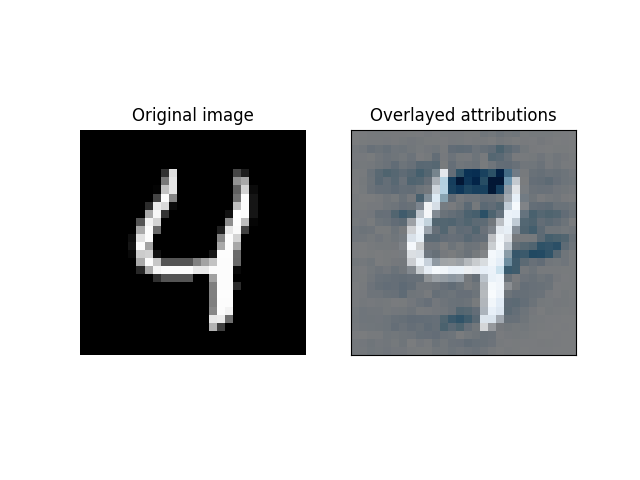
\includegraphics[width=.6\linewidth]{img/saliency_mnist/4.png}
    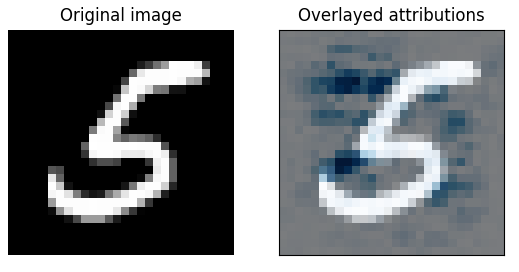
\includegraphics[width=.6\linewidth]{img/saliency_mnist/5.png}
    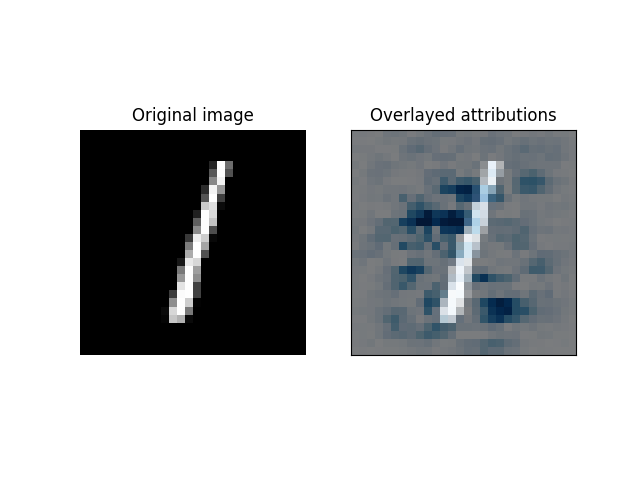
\includegraphics[width=.6\linewidth]{img/saliency_mnist/1.png}
    \caption{Saliency maps of chosen MNIST digits}\label{fig:mnist-cnn-saliency}
\end{figure}

The CNN for recognizing handwritten digits from the MNIST dataset was analyzed using the saliency methods.
The resulting saliency maps are visualized on fig.~\ref{fig:mnist-cnn-saliency}.
The blue pixels show the areas that most influence the model's predictions.

Unexpectedly, the obtained saliency maps predominantly highlight background pixels adjacent to the digits
rather than the digits themselves.
One plausible explanation of this phenomenon is that the CNN has learned the absence of pixels in a specific region as
important information for its classification decisions --- for example, the digits 4 and 5 are characterized by the lack of the closed regions.
If one was to add pixels to these areas 4 would turn into a 9, and 5 would turn into a 6.
Therefore, these areas are highlighted as important to the classification results, because it is essential that no pixels exist in those areas.
Such behaviour might suggest that the model is not recognizing the digits by their shape directly, but rather by elimination --- i.e.\ an important characteristic of a digit 4 is that it is not a 9.

The background pixels might also provide contextual information about the area around the digit.
This is especially important in shape recognition tasks, such as digit recognition.
For example, the top bar at the digit 5 is oriented to the right-hand side, however, there are pixels highlighted to the left-hand side.
That is because for a line to be considered as oriented to the right, there need to be both a presence of pixels to the right, and a lack of them to the left.
Therefore, the background also needs to be considered in order to correctly determine the shape characteristics and boundaries.

Another unfortunate possibility of such behaviour may be some issues with the model.
Overfitting could cause the model to focus on some background pixels, that are not really representative of the digit features.
However, it should be noted that during the model evaluation, we did not observe a drop in accuracy on the test set during training --- a typical sign of overfitting.
Additionally, the performance of the model on the testing data was satisfactory, which speaks against the potential issues with the model.

To further investigate this model we used Integrated Gradients method as well.
\begin{figure}[h]\centering
    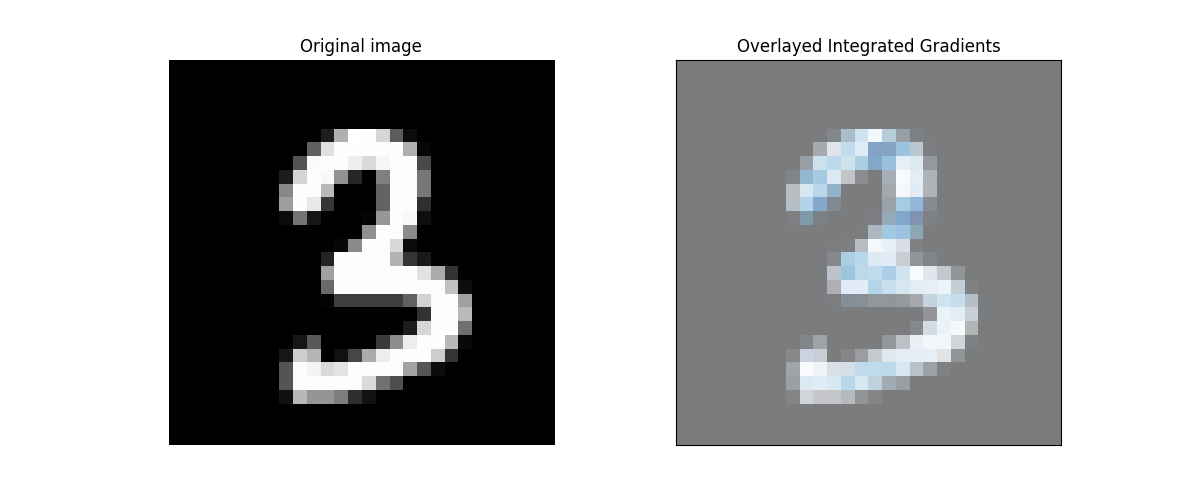
\includegraphics[width=.6\linewidth]{img/integrated_grad/mnist_CNN/3}
    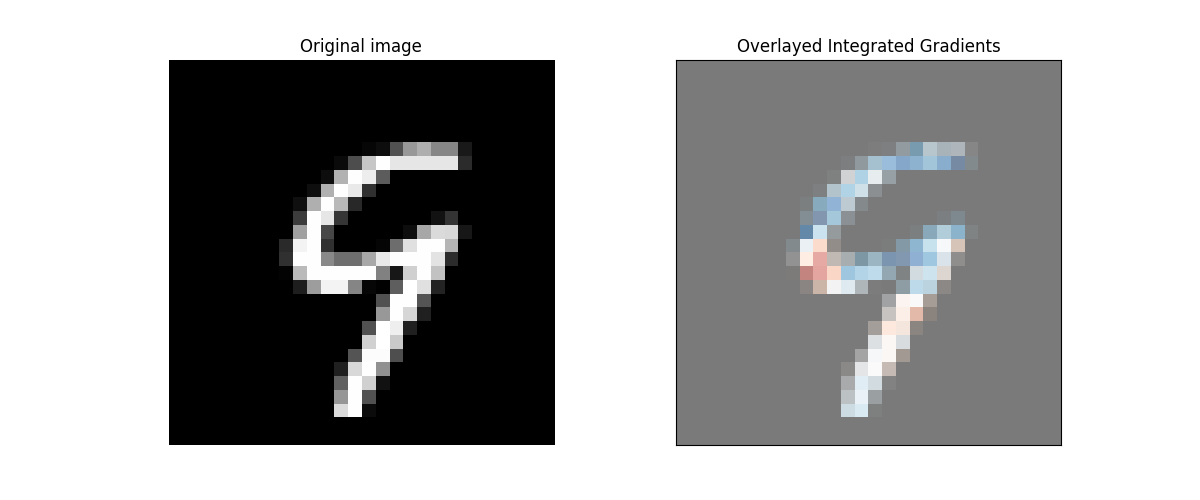
\includegraphics[width=.6\linewidth]{img/integrated_grad/mnist_CNN/4_again2}
    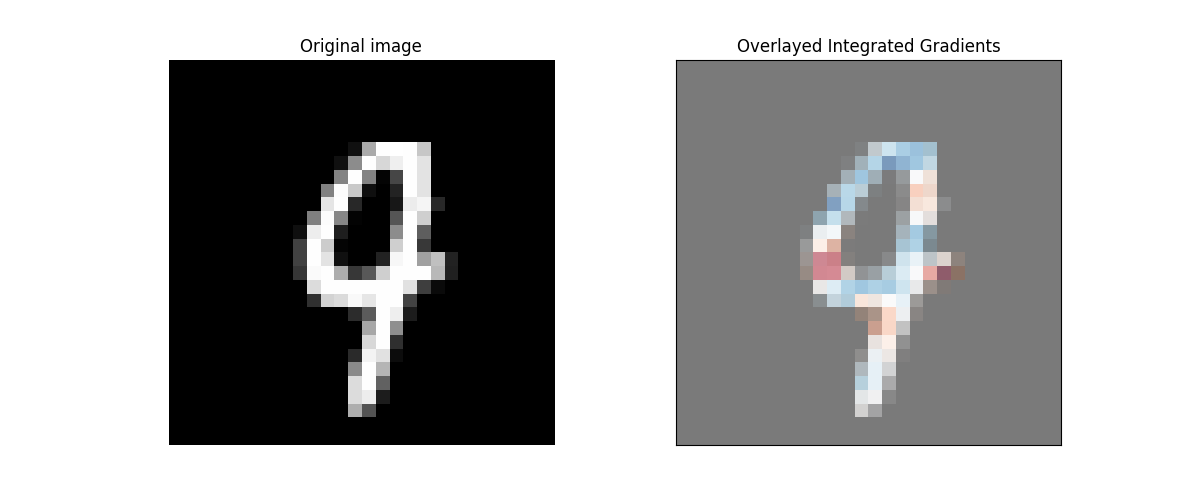
\includegraphics[width=.6\linewidth]{img/integrated_grad/mnist_CNN/9}
    \caption{Integrated Gradients of chosen MNIST digits}\label{fig:mnist-cnn-integrated-grad}
\end{figure}
As previously the blue pixels show the areas that most influence the model's predictions and red the least.

Obtained integrated gradients perfectly present and explain which areas are taken into account when predicting by a model.
Examples on fig.~\ref{fig:mnist-cnn-integrated-grad} show that digit 3 is most recognizable by its' two distinctive curves.
This insight aligns with human intuition about the defining features of the numeral 3.
Integrated Gradients also reveal nuances in distinguishing between visually similar digits.
For digits 4 and 9, while they share some similarities, the connected top part plays a critical role in differentiation.
Moreover, this method highlight areas in the digits where the model might make errors or find ambiguity.
In the central areas of digits 4 and 9, represented by less intense colors (notably red), the model's certainty decreases.
This suggests these regions resemble characteristics of multiple digits, potentially leading to misclassification.

We extended our analysis by implementing the SLIC superpixel method.

\begin{figure}[h]\centering
    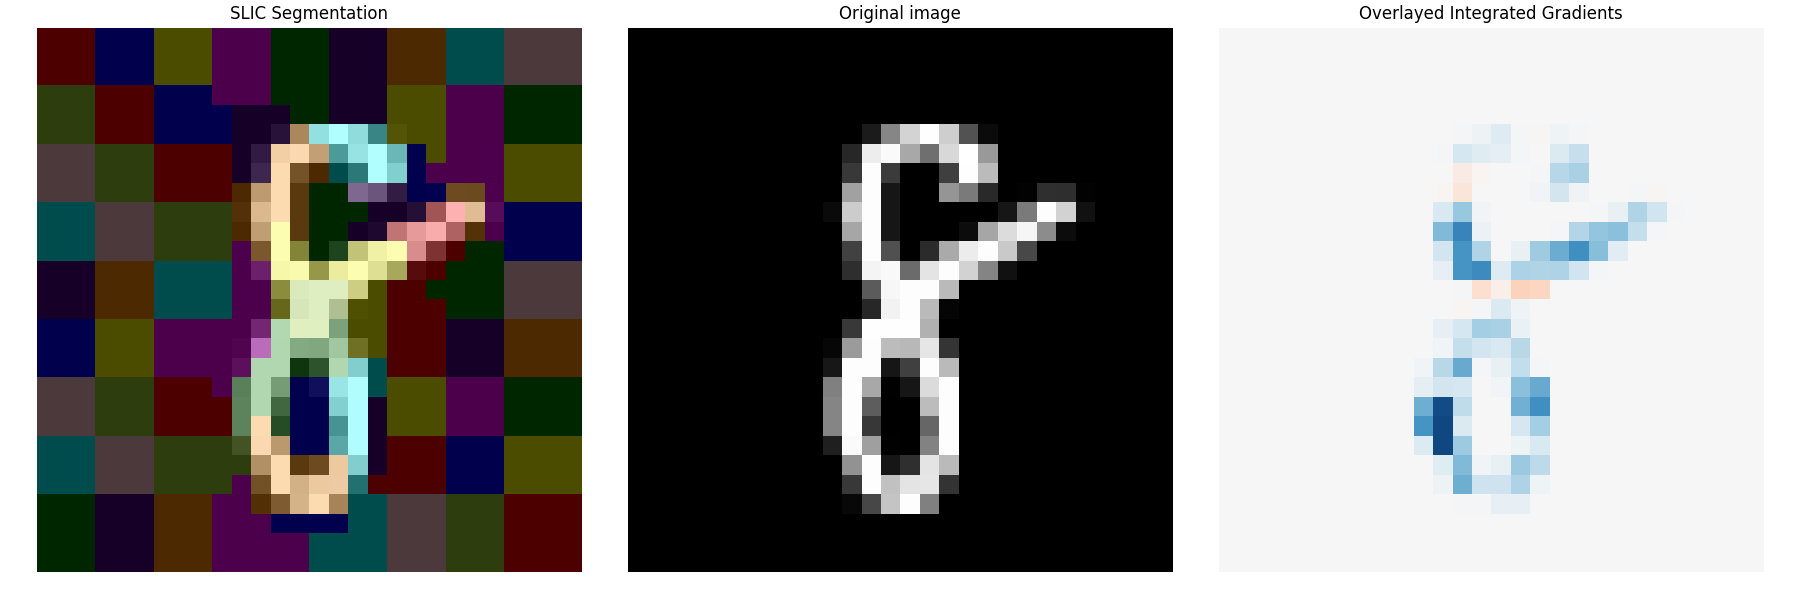
\includegraphics[width=.6\linewidth]{img/SLIC/mnist/8}
    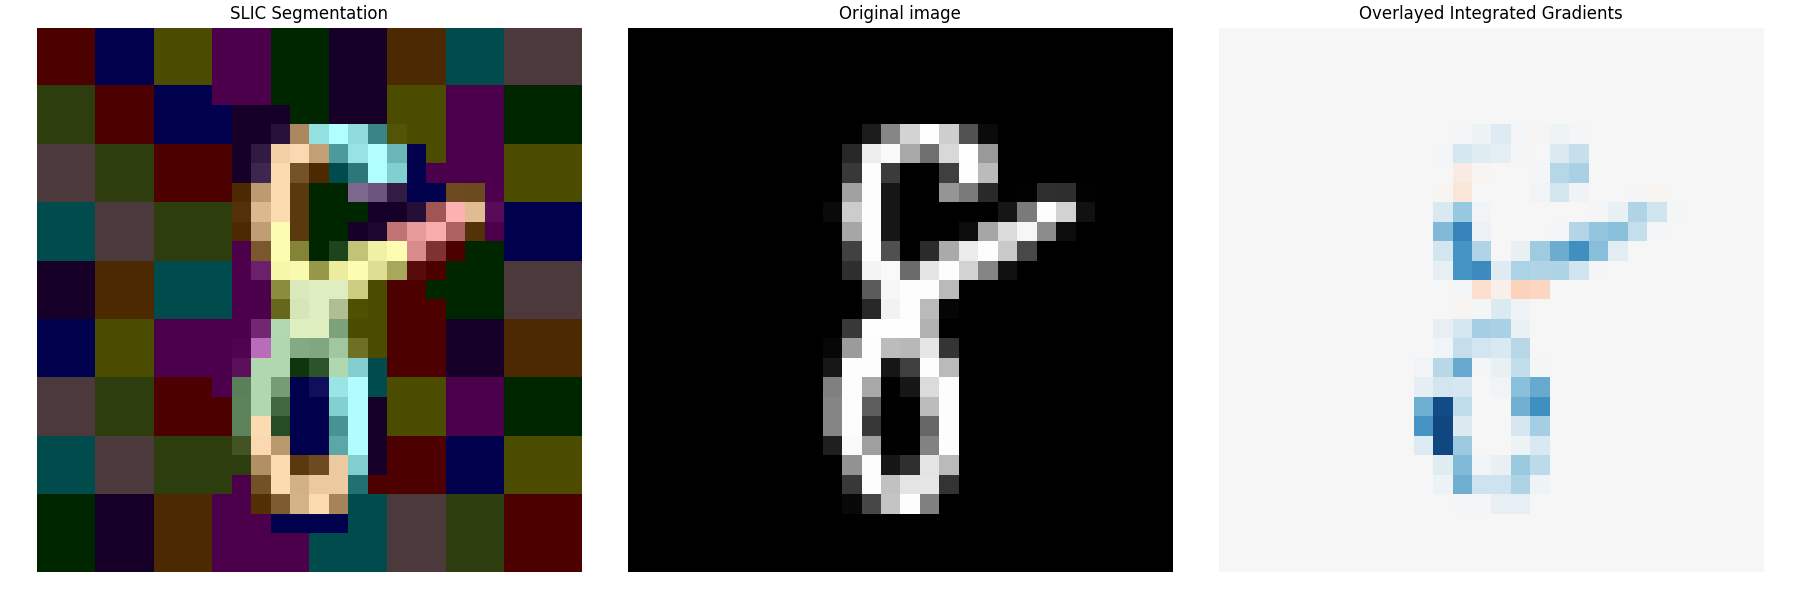
\includegraphics[width=.6\linewidth]{img/SLIC/mnist/8_1}
    \caption{SLIC method on chosen MNIST digits}\label{fig:mnist-cnn-slic}
\end{figure}

SLIC generates segmented regions that highlight the spatial importance of different parts of the digit.
By focusing on these superpixels, we gain insights into which regions the model prioritizes when making decisions.
For example on the fig.~\ref{fig:mnist-cnn-slic} we observe that in case of classification fo difit 8, the most crucial part is the center, where two curves cross each other.
Integrating this method enhances model transparency and improves understanding of the model prediction.

At last, we used peturbation technique on different digits to check, how model would classify them, if part of the image would be covered.

\begin{figure}[ht]\centering
    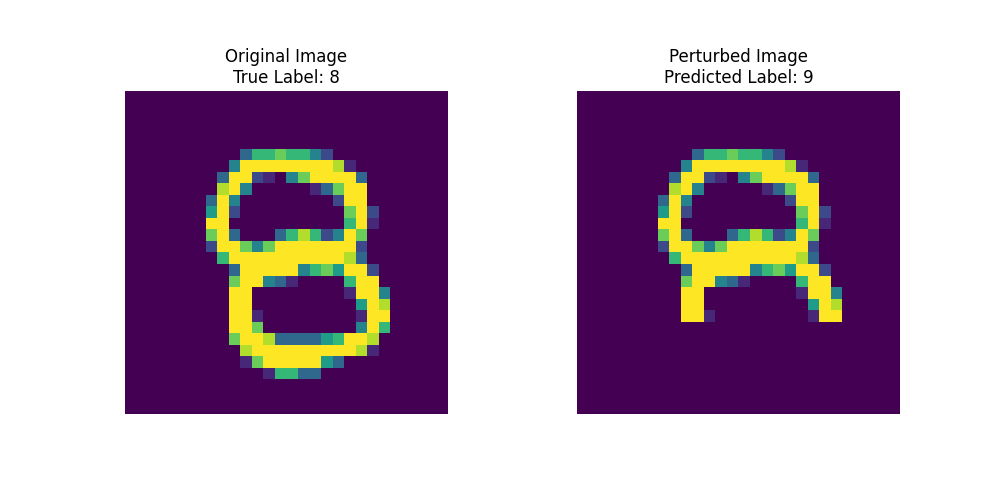
\includegraphics[width=.6\linewidth]{img/counterfacts/MNIST/cover_bottom/img_1}
    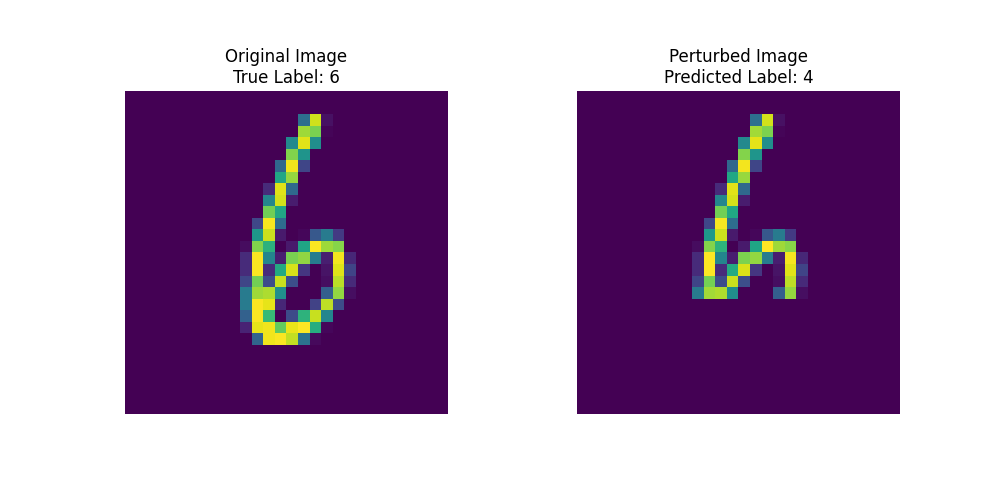
\includegraphics[width=.6\linewidth]{img/counterfacts/MNIST/cover_bottom/img_3}
    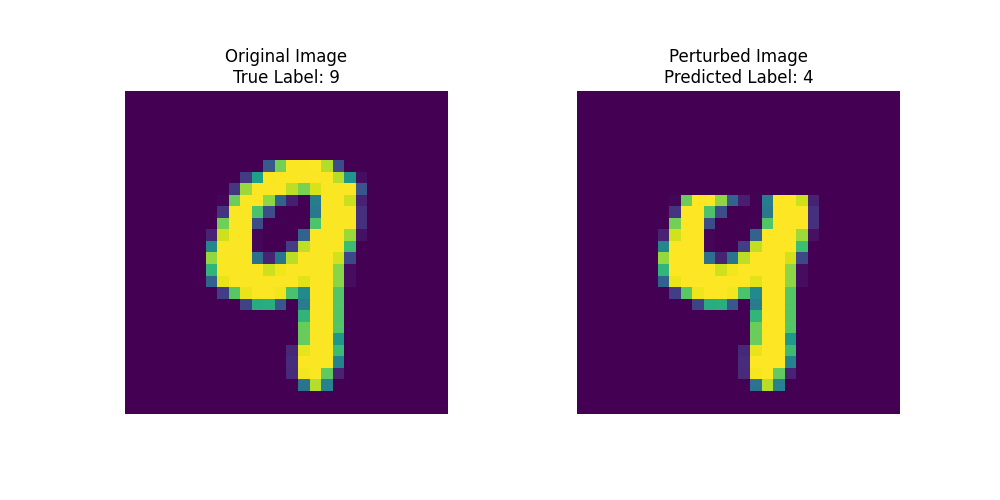
\includegraphics[width=.6\linewidth]{img/counterfacts/MNIST/cover_top/img_10}
    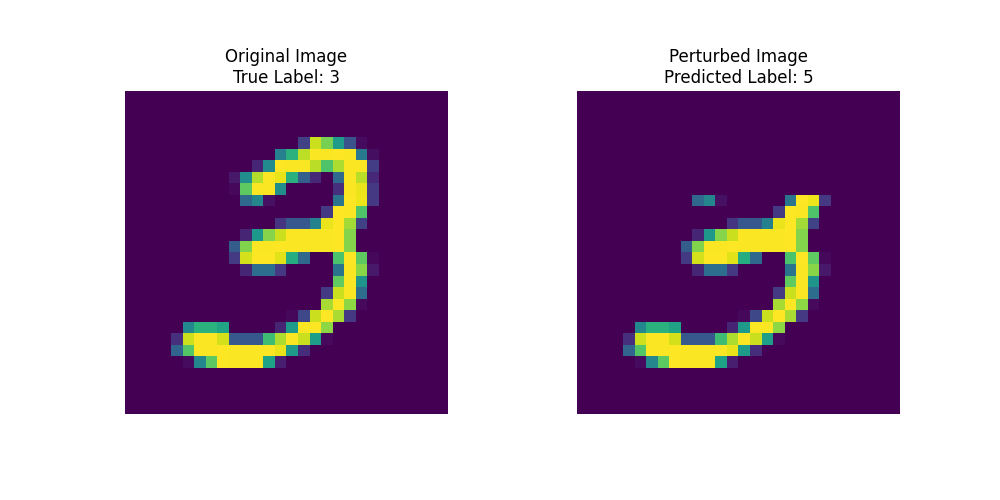
\includegraphics[width=.6\linewidth]{img/counterfacts/MNIST/cover_top/img_3}
    \caption{Peturbation method on chosen MNIST digits}\label{fig:mnist-cnn-counterfacts}
\end{figure}

We can observe on the fig.~\ref{fig:mnist-cnn-counterfacts} that covering the bottom part of the digit 8 leads the model to classify it as 9.
Similarly, covering part of the digit 6 results in a misclassification as 4.
These observations highlight specific regions of the image that significantly influence the model's predictions.
The perfect example of explanation of the figures on ~\ref{fig:mnist-cnn-integrated-grad} is with the coverage of the top part of 9, which results in misclassification as 4.
Therefore, it proves the fact that the top part of digit 9 is most influential.
Same results are obtained on the last example, where instead of predicting 3, model predicts 5 due to lack of the top curve.

This technique is a powerful tool for error analysis and diagnosis.
Using it demonstrates how small changes in input can affect model predictions and trustworthiness.

\subsection{CIFAR10 CNN classifier}\label{subsec:experiment-cifar}

\begin{figure}[ht]\centering
    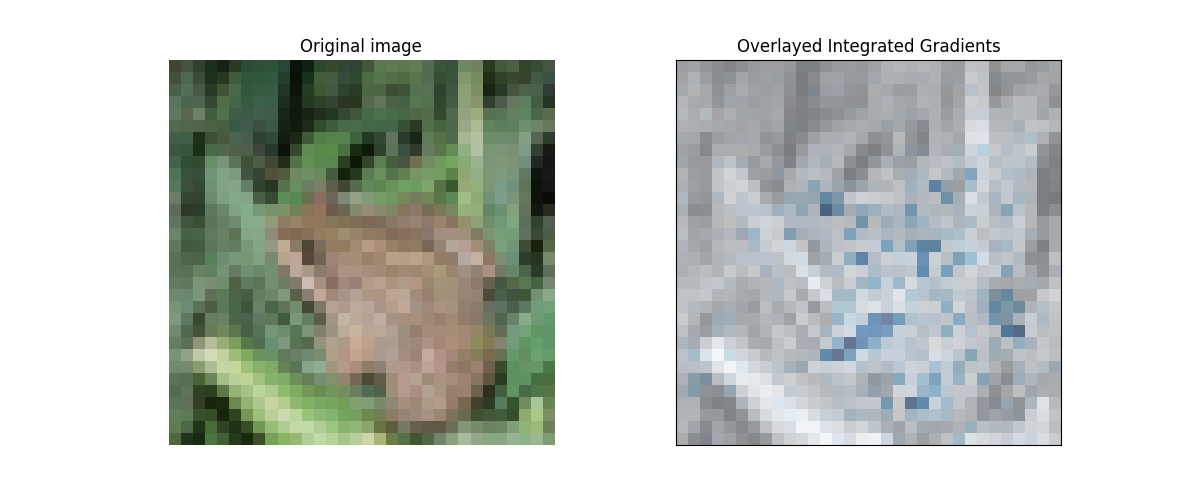
\includegraphics[width=.6\linewidth]{img/integrated_grad/cifar_CNN/frog}
    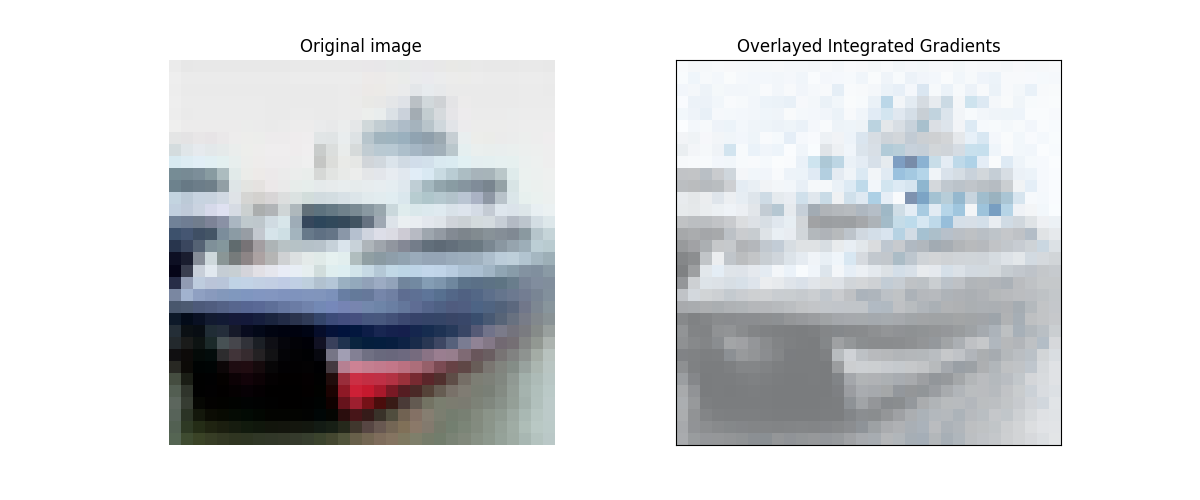
\includegraphics[width=.6\linewidth]{img/integrated_grad/cifar_CNN/ship}
    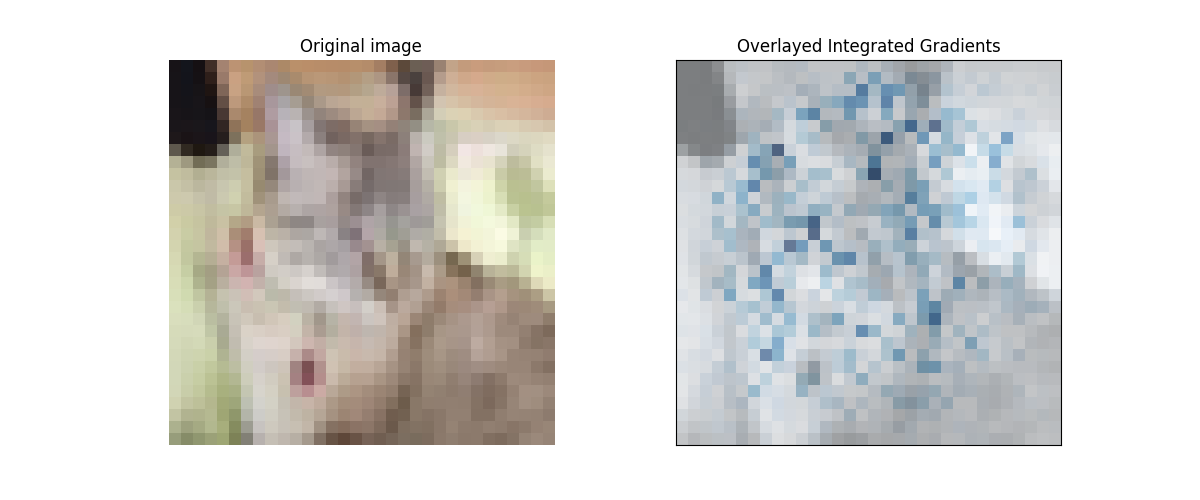
\includegraphics[width=.6\linewidth]{img/integrated_grad/cifar_CNN/cat2}
    \caption{Integrated Gradients of chosen CIFAR images}\label{fig:cifar-cnn-int-grad}
\end{figure}
In our exploration of CNN model trained on the CIFAR10 dataset, we utilized Integrated Gradients to enhance our understanding of how these models classify objects within images.

Integrated Gradients highlight significant object features within CIFAR10 images, offering valuable insights into the model's decision-making process.
This focus is particularly effective for images where objects are distinct and prominently displayed, such as the frog and cat examples on fig.~\ref{fig:cifar-cnn-int-grad}.
Here, the model accurately identifies and highlights features of these objects, enhancing interpretability.
However, challenges arise with images like the ship, where the object’s distinction from the background is less pronounced.
In such cases, Integrated Gradients struggle to clearly delineate object boundaries due to color similarity or background complexity.

Addressing this challenge with background interference may involve enhancing model robustness through data augmentation or adapting interpretability techniques tailored to complex visual environments.
Such insights are crucial for deploying CNN models in real-world scenarios, such as autonomous systems, medical diagnostics, and security surveillance, where accurate object recognition amidst varying environmental conditions is paramount.

To further investigate model prediction, we implemented the SLIC super-pixel method.
IS IT OK??
\begin{figure}[ht]\centering
    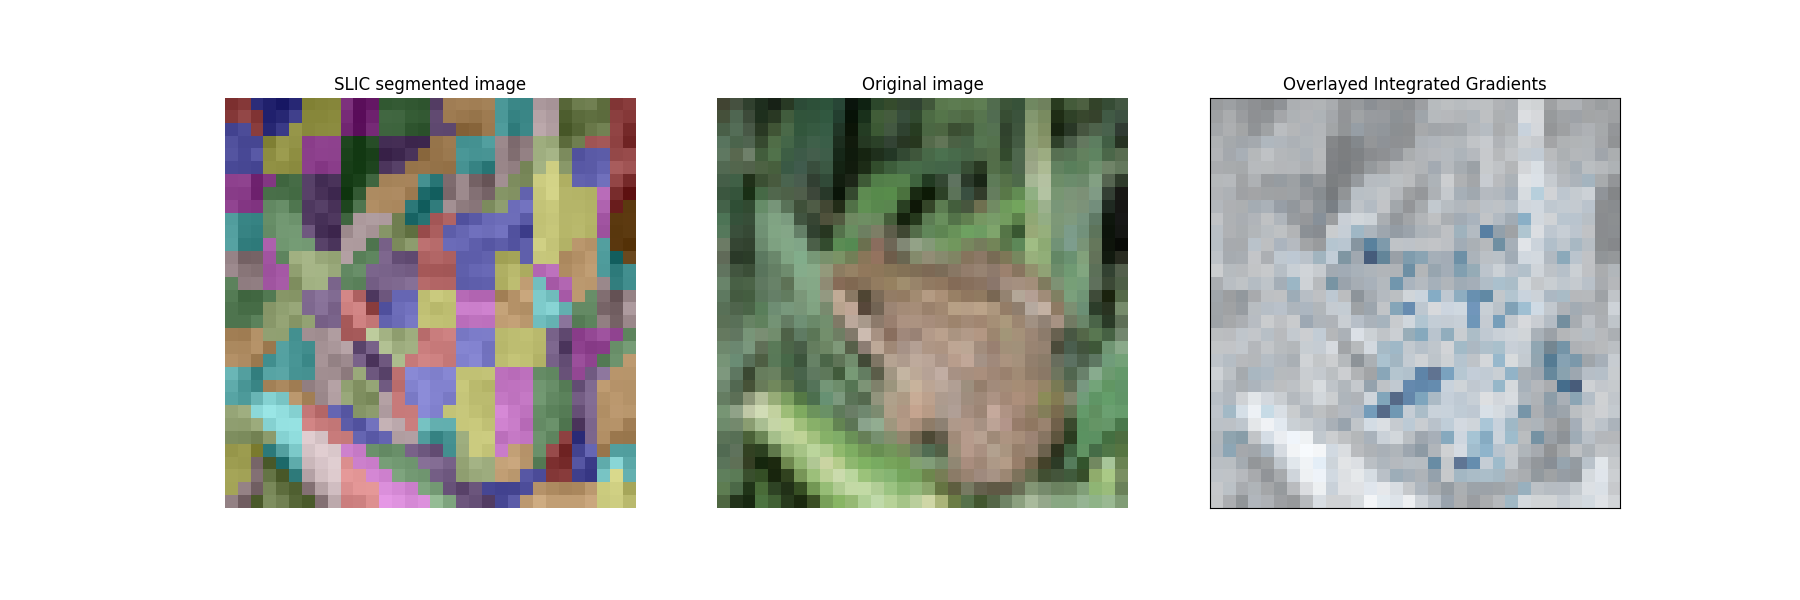
\includegraphics[width=.6\linewidth]{img/SLIC/cifar/img_5}
    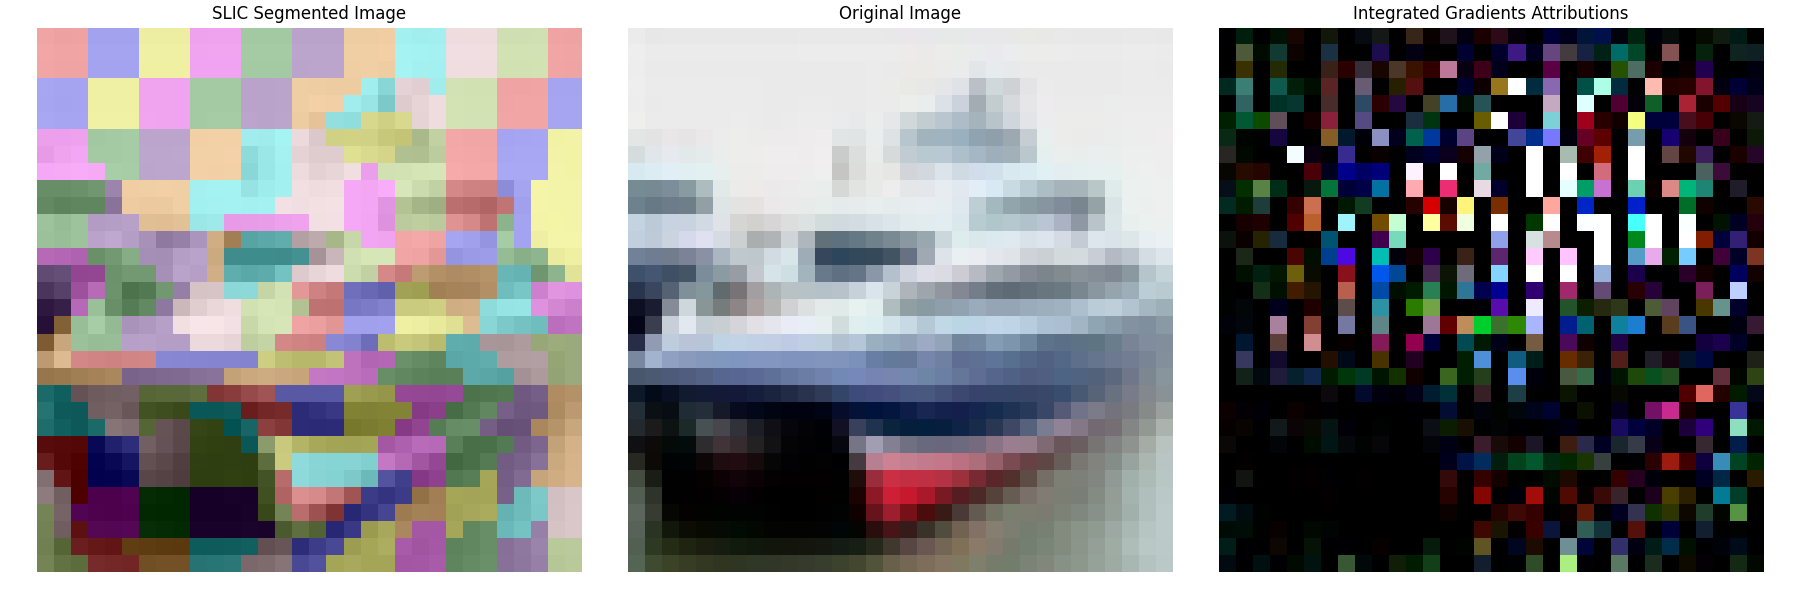
\includegraphics[width=.6\linewidth]{img/SLIC/cifar/img_6}
    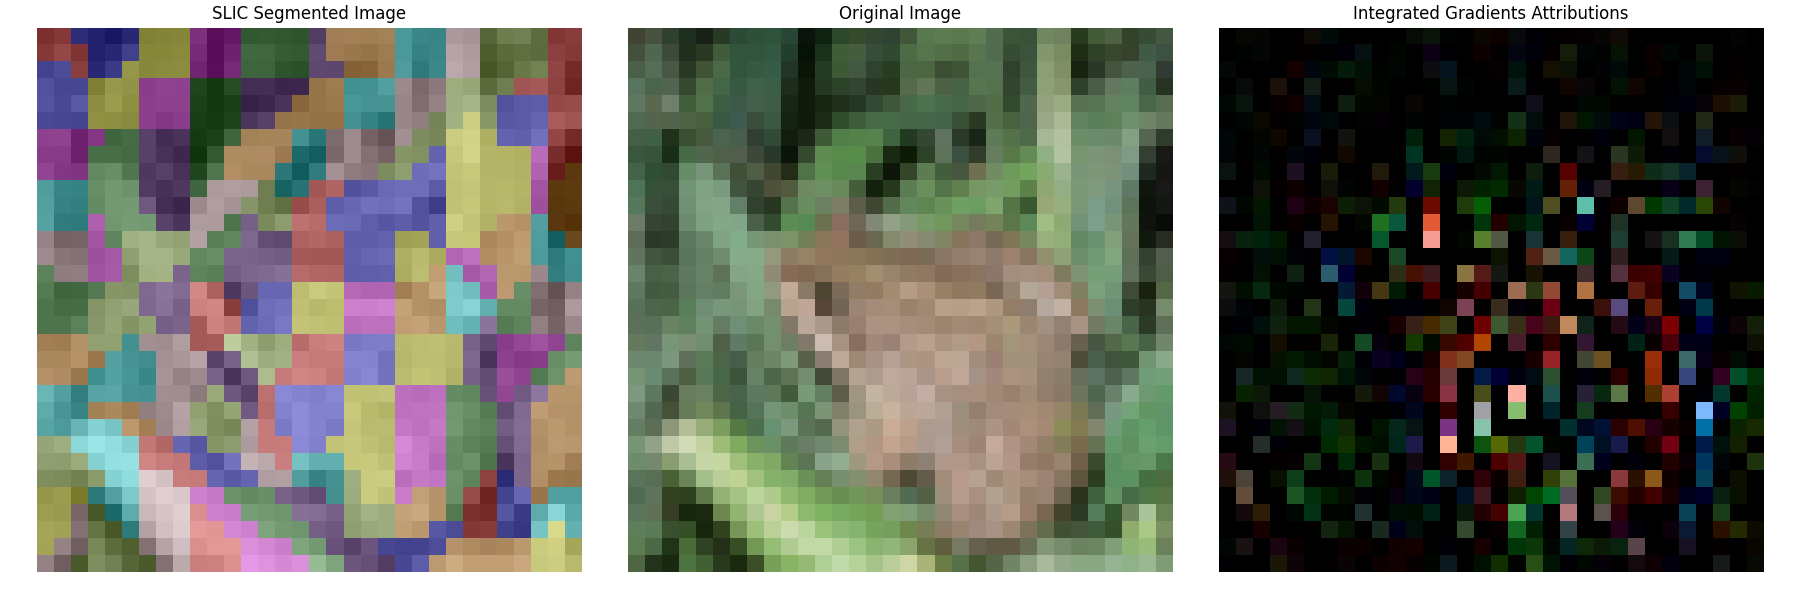
\includegraphics[width=.6\linewidth]{img/SLIC/cifar/img_9}
    \caption{SLIC method on chosen CIFAR images}\label{fig:cifar-cnn-slic}
\end{figure}

To further assess the robustness and reliability of our CNN model trained on the CIFAR10 dataset, we implemented perturbation techniques.
Specifically, we investigated how the model's classification performance changes when images are slightly rotated.
This analysis helps us understand the model's sensitivity to variations in input and its reliance on specific visual features for accurate predictions.

\begin{figure}[ht]\centering
    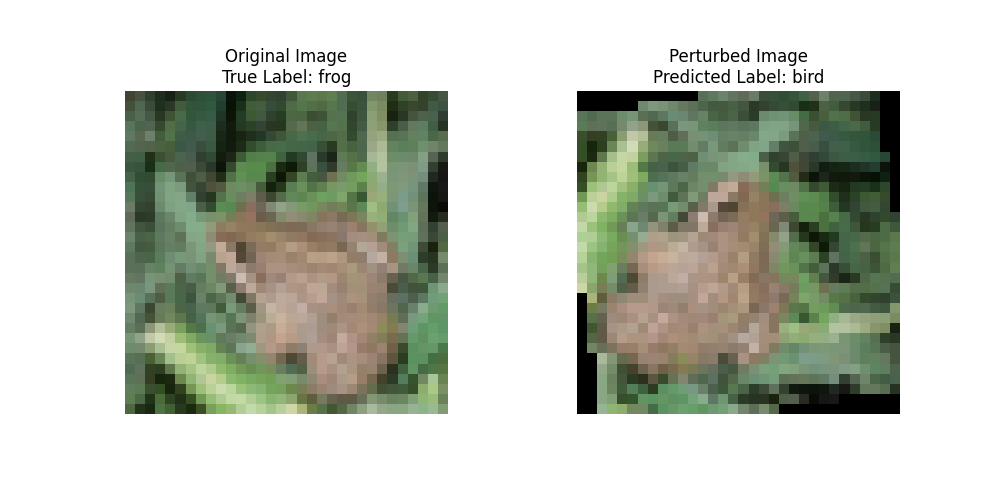
\includegraphics[width=.6\linewidth]{img/counterfacts/CIFAR/img_2}
    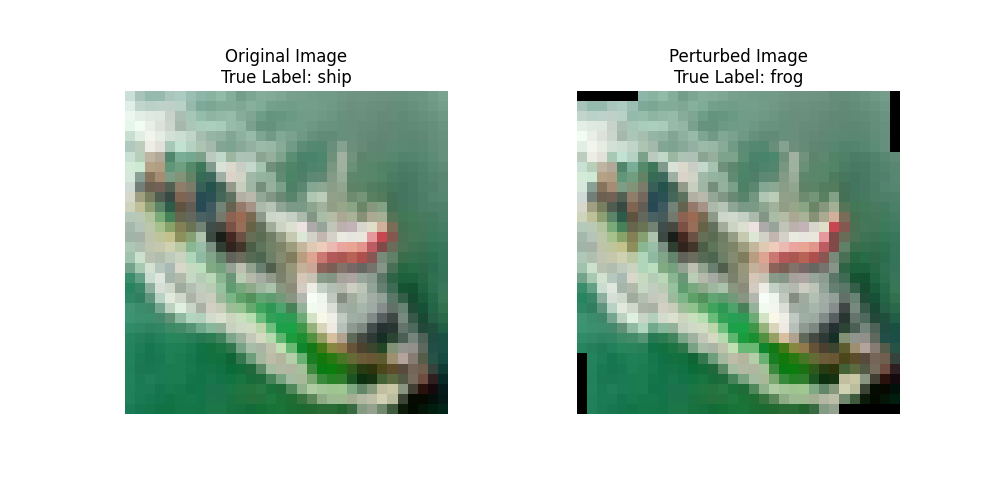
\includegraphics[width=.6\linewidth]{img/counterfacts/CIFAR/img_7}
    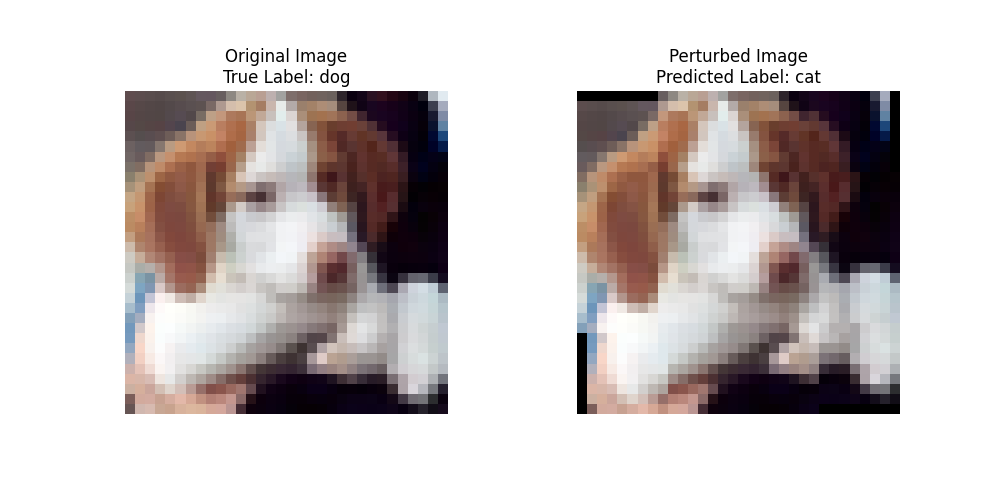
\includegraphics[width=.6\linewidth]{img/counterfacts/CIFAR/img_8}
    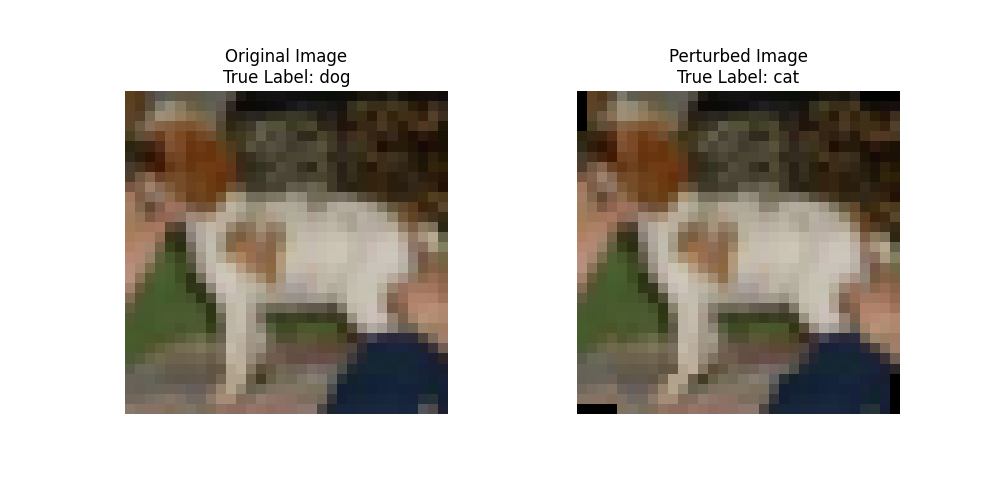
\includegraphics[width=.6\linewidth]{img/counterfacts/CIFAR/img_6}
    \caption{Peturbation on chosen CIFAR images}\label{fig:cifar-cnn-peturbation}
\end{figure}

The perturbation results, depicted on fig.~\ref{fig:cifar-cnn-peturbation}, provide a detailed view of the model's behavior under rotational transformations.
For images where the object of interest is prominently displayed and distinct from the background, the model demonstrates robustness to significant rotations.
For instance, the frog image requires a rotation above 82.15 degrees before the model misclassifies it.
This indicates that the model reliably recognizes the frog based on its salient features despite substantial perturbations.

However, images with less distinct objects or complex backgrounds show vulnerability to even minor rotations.
The ship image, for instance, is misclassified as a frog with only a 3.65-degree rotation.
This misclassification likely arises due to the green background, which the model mistakenly associates with the frog class.
This scenario highlights the model's susceptibility to background interference when object and background colors are similar.
The model also shows difficulty distinguishing between visually similar classes under slight perturbations.
As seen on fig.~\ref{fig:cifar-cnn-peturbation}, small rotations (2.47 and 3.85 degrees) cause the model to misclassify a dog as a cat.
This suggests that the model's feature extraction process may not effectively differentiate between subtle visual differences in closely related classes.

These findings underscore the importance of rigorous model evaluation under diverse conditions to ensure reliability in practical applications.
Models deployed in different fields such as surveillance or medical imaging must maintain high accuracy despite variations in input, making perturbation analysis a critical component of model validation.

Addressing this challenge through targeted training enhancements and interpretability techniques can lead to more robust and reliable models suited for complex real-world tasks.

\section{Summary}\label{sec:summary}
Summarize the main conclusions and suggest future work.

\section{References}\label{sec:references}

\bibliographystyle{IEEEtran}
\bibliography{references}

\end{document}
